\documentclass[preview]{standalone}

\usepackage{amsmath}
\usepackage{amssymb}
\usepackage{stellar}
\usepackage{definitions}
\usepackage{tikz}

\usetikzlibrary{calc}
\usetikzlibrary{decorations.markings}
\usetikzlibrary{cd}

\begin{document}

\id{konigsberg-bridges}
\genpage

\section{The Königsberg Bridges Problem}

\begin{snippet}{konigsberg-bridges-explanation}
    The Königsberg bridges problem consists in determining whether it is possible to take a walk that crosses each bridge exactly once, possibly returning to the starting point.
    The fundamental idea is that the precise shape of the regions or bridges does not matter: what matters is only which regions are connected by which bridges. We therefore represent the regions with points, called \emph{vertices}, and the bridges with arcs, called \emph{edges}.
    This graph is not simple: there may be multiple bridges between two regions, so multiple edges appear in the graph.
\end{snippet}

\begin{snippet}{konigsberg-bridges-illustration}
    \begin{center}
        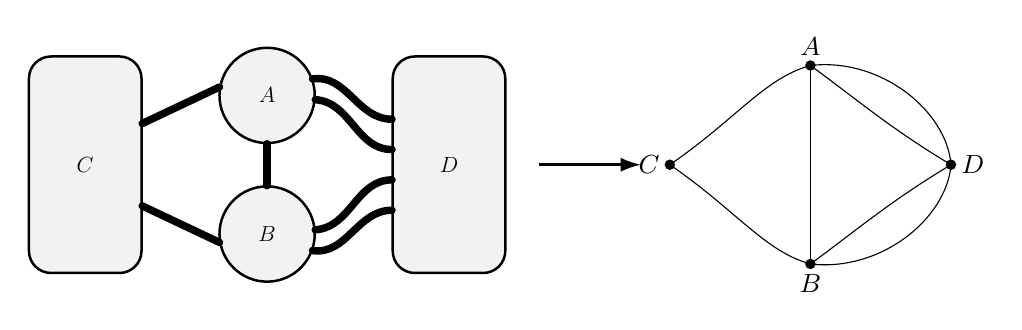
\begin{tikzpicture}[
            >=Latex,
            every node/.style={font=\small},
            land/.style={draw=black, line width=0.9pt, fill=gray!10},
            bridge/.style={
                draw=black,
                double=black,
                double distance=2pt,
                line width=0.35pt,
                line cap=round
            }
        ]

        \begin{scope}[scale=0.55, transform shape]
            \node[land, rounded corners=8pt,
                minimum width=2.6cm, minimum height=5.0cm] (LC) at (-4.2,0) {};

            \node[land, circle, minimum size=2.2cm] (LA) at (0,1.6) {};

            \node[land, circle, minimum size=2.2cm] (LB) at (0,-1.6) {};

            \node[land, rounded corners=8pt,
                minimum width=2.6cm, minimum height=5.0cm] (LD) at (4.2,0) {};

            \coordinate (LCA)  at ($(LC.east)+(0,0.95)$);
            \coordinate (LCB)  at ($(LC.east)+(0,-0.95)$);

            \coordinate (LDAu) at ($(LD.west)+(0,1.05)$);
            \coordinate (LDAl) at ($(LD.west)+(0,0.35)$);
            \coordinate (LDBu) at ($(LD.west)+(0,-0.35)$);
            \coordinate (LDBl) at ($(LD.west)+(0,-1.05)$);

            \draw[bridge] (LCA) -- (LA.170);
            \draw[bridge] (LCB) -- (LB.190);
            \draw[bridge] (LA.-90) -- (LB.90);

            \draw[bridge] (LA.20)  to[out=8,in=180]  (LDAu);
            \draw[bridge] (LA.-5)  to[out=-4,in=180] (LDAl);

            \draw[bridge] (LB.5)   to[out=4,in=180]  (LDBu);
            \draw[bridge] (LB.-20) to[out=-8,in=180] (LDBl);

            \node at (LC) {\Large \(C\)};
            \node at (LA) {\Large \(A\)};
            \node at (LB) {\Large \(B\)};
            \node at (LD) {\Large \(D\)};
        \end{scope}

        \draw[line width=0.9pt, -{Latex[length=2.6mm,width=1.8mm]}]
            (3.45,0) -- (4.75,0);

        \begin{scope}[xshift=6.9cm, scale=1.05, transform shape]
            \coordinate (RA) at (0,1.2);
            \coordinate (RB) at (0,-1.2);
            \coordinate (RC) at (-1.7,0);
            \coordinate (RD) at (1.7,0);

            \fill (RA) circle (1.8pt);
            \fill (RB) circle (1.8pt);
            \fill (RC) circle (1.8pt);
            \fill (RD) circle (1.8pt);

            \node[above] at (RA) {\(A\)};
            \node[below] at (RB) {\(B\)};
            \node[left]  at (RC) {\(C\)};
            \node[right] at (RD) {\(D\)};

            \draw (RC) .. controls (-0.9,0.55) and (-0.55,1.05) .. (RA);
            \draw (RC) .. controls (-0.9,-0.55) and (-0.55,-1.05) .. (RB);

            \draw (RA) .. controls (0.55,0.8) and (0.95,0.45) .. (RD);
            \draw (RA) .. controls (0.85,1.3) and (1.65,0.65) .. (RD);

            \draw (RB) .. controls (0.55,-0.8) and (0.95,-0.45) .. (RD);
            \draw (RB) .. controls (0.85,-1.3) and (1.65,-0.65) .. (RD);

            \draw (RA) -- (RB);
        \end{scope}

        \end{tikzpicture}
    \end{center}
\end{snippet}

\end{document}